% Created by tikzDevice version 0.12.3 on 2020-05-28 00:34:20
% !TEX encoding = UTF-8 Unicode
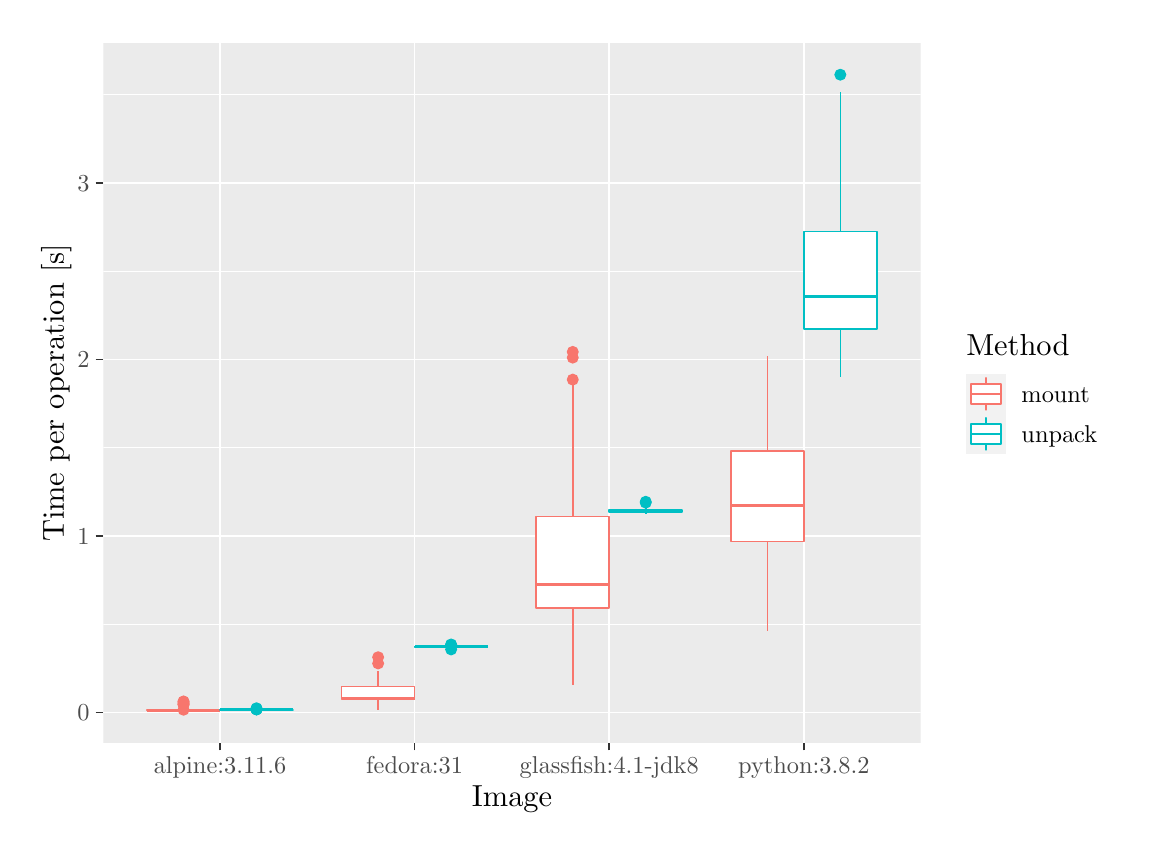
\begin{tikzpicture}[x=1pt,y=1pt]
\definecolor{fillColor}{RGB}{255,255,255}
\path[use as bounding box,fill=fillColor,fill opacity=0.00] (0,0) rectangle (397.48,289.08);
\begin{scope}
\path[clip] (  0.00,  0.00) rectangle (397.48,289.08);
\definecolor{drawColor}{RGB}{255,255,255}
\definecolor{fillColor}{RGB}{255,255,255}

\path[draw=drawColor,line width= 0.6pt,line join=round,line cap=round,fill=fillColor] (  0.00,  0.00) rectangle (397.48,289.08);
\end{scope}
\begin{scope}
\path[clip] ( 27.31, 30.69) rectangle (322.66,283.58);
\definecolor{fillColor}{gray}{0.92}

\path[fill=fillColor] ( 27.31, 30.69) rectangle (322.66,283.58);
\definecolor{drawColor}{RGB}{255,255,255}

\path[draw=drawColor,line width= 0.3pt,line join=round] ( 27.31, 73.55) --
	(322.66, 73.55);

\path[draw=drawColor,line width= 0.3pt,line join=round] ( 27.31,137.34) --
	(322.66,137.34);

\path[draw=drawColor,line width= 0.3pt,line join=round] ( 27.31,201.12) --
	(322.66,201.12);

\path[draw=drawColor,line width= 0.3pt,line join=round] ( 27.31,264.91) --
	(322.66,264.91);

\path[draw=drawColor,line width= 0.6pt,line join=round] ( 27.31, 41.66) --
	(322.66, 41.66);

\path[draw=drawColor,line width= 0.6pt,line join=round] ( 27.31,105.44) --
	(322.66,105.44);

\path[draw=drawColor,line width= 0.6pt,line join=round] ( 27.31,169.23) --
	(322.66,169.23);

\path[draw=drawColor,line width= 0.6pt,line join=round] ( 27.31,233.02) --
	(322.66,233.02);

\path[draw=drawColor,line width= 0.6pt,line join=round] ( 69.51, 30.69) --
	( 69.51,283.58);

\path[draw=drawColor,line width= 0.6pt,line join=round] (139.83, 30.69) --
	(139.83,283.58);

\path[draw=drawColor,line width= 0.6pt,line join=round] (210.15, 30.69) --
	(210.15,283.58);

\path[draw=drawColor,line width= 0.6pt,line join=round] (280.47, 30.69) --
	(280.47,283.58);
\definecolor{drawColor}{RGB}{248,118,109}
\definecolor{fillColor}{RGB}{248,118,109}

\path[draw=drawColor,line width= 0.4pt,line join=round,line cap=round,fill=fillColor] ( 56.32, 42.61) circle (  1.96);

\path[draw=drawColor,line width= 0.4pt,line join=round,line cap=round,fill=fillColor] ( 56.32, 44.61) circle (  1.96);

\path[draw=drawColor,line width= 0.4pt,line join=round,line cap=round,fill=fillColor] ( 56.32, 44.54) circle (  1.96);

\path[draw=drawColor,line width= 0.4pt,line join=round,line cap=round,fill=fillColor] ( 56.32, 45.57) circle (  1.96);

\path[draw=drawColor,line width= 0.4pt,line join=round,line cap=round,fill=fillColor] ( 56.32, 45.58) circle (  1.96);

\path[draw=drawColor,line width= 0.4pt,line join=round,line cap=round,fill=fillColor] ( 56.32, 44.51) circle (  1.96);

\path[draw=drawColor,line width= 0.4pt,line join=round,line cap=round,fill=fillColor] ( 56.32, 45.20) circle (  1.96);

\path[draw=drawColor,line width= 0.6pt,line join=round] ( 56.32, 42.43) -- ( 56.32, 42.57);

\path[draw=drawColor,line width= 0.6pt,line join=round] ( 56.32, 42.33) -- ( 56.32, 42.18);
\definecolor{fillColor}{RGB}{255,255,255}

\path[draw=drawColor,line width= 0.6pt,line join=round,line cap=round,fill=fillColor] ( 43.14, 42.43) --
	( 43.14, 42.33) --
	( 69.51, 42.33) --
	( 69.51, 42.43) --
	( 43.14, 42.43) --
	cycle;

\path[draw=drawColor,line width= 1.1pt,line join=round] ( 43.14, 42.38) -- ( 69.51, 42.38);
\definecolor{drawColor}{RGB}{0,191,196}
\definecolor{fillColor}{RGB}{0,191,196}

\path[draw=drawColor,line width= 0.4pt,line join=round,line cap=round,fill=fillColor] ( 82.69, 43.16) circle (  1.96);

\path[draw=drawColor,line width= 0.4pt,line join=round,line cap=round,fill=fillColor] ( 82.69, 42.77) circle (  1.96);

\path[draw=drawColor,line width= 0.4pt,line join=round,line cap=round,fill=fillColor] ( 82.69, 42.79) circle (  1.96);

\path[draw=drawColor,line width= 0.4pt,line join=round,line cap=round,fill=fillColor] ( 82.69, 42.78) circle (  1.96);

\path[draw=drawColor,line width= 0.4pt,line join=round,line cap=round,fill=fillColor] ( 82.69, 42.81) circle (  1.96);

\path[draw=drawColor,line width= 0.4pt,line join=round,line cap=round,fill=fillColor] ( 82.69, 42.79) circle (  1.96);

\path[draw=drawColor,line width= 0.4pt,line join=round,line cap=round,fill=fillColor] ( 82.69, 42.79) circle (  1.96);

\path[draw=drawColor,line width= 0.4pt,line join=round,line cap=round,fill=fillColor] ( 82.69, 42.74) circle (  1.96);

\path[draw=drawColor,line width= 0.6pt,line join=round] ( 82.69, 42.63) -- ( 82.69, 42.68);

\path[draw=drawColor,line width= 0.6pt,line join=round] ( 82.69, 42.56) -- ( 82.69, 42.54);
\definecolor{fillColor}{RGB}{255,255,255}

\path[draw=drawColor,line width= 0.6pt,line join=round,line cap=round,fill=fillColor] ( 69.51, 42.63) --
	( 69.51, 42.56) --
	( 95.88, 42.56) --
	( 95.88, 42.63) --
	( 69.51, 42.63) --
	cycle;

\path[draw=drawColor,line width= 1.1pt,line join=round] ( 69.51, 42.58) -- ( 95.88, 42.58);
\definecolor{drawColor}{RGB}{248,118,109}
\definecolor{fillColor}{RGB}{248,118,109}

\path[draw=drawColor,line width= 0.4pt,line join=round,line cap=round,fill=fillColor] (126.64, 61.60) circle (  1.96);

\path[draw=drawColor,line width= 0.4pt,line join=round,line cap=round,fill=fillColor] (126.64, 59.35) circle (  1.96);

\path[draw=drawColor,line width= 0.6pt,line join=round] (126.64, 51.02) -- (126.64, 56.48);

\path[draw=drawColor,line width= 0.6pt,line join=round] (126.64, 46.44) -- (126.64, 42.37);
\definecolor{fillColor}{RGB}{255,255,255}

\path[draw=drawColor,line width= 0.6pt,line join=round,line cap=round,fill=fillColor] (113.46, 51.02) --
	(113.46, 46.44) --
	(139.83, 46.44) --
	(139.83, 51.02) --
	(113.46, 51.02) --
	cycle;

\path[draw=drawColor,line width= 1.1pt,line join=round] (113.46, 46.56) -- (139.83, 46.56);
\definecolor{drawColor}{RGB}{0,191,196}
\definecolor{fillColor}{RGB}{0,191,196}

\path[draw=drawColor,line width= 0.4pt,line join=round,line cap=round,fill=fillColor] (153.01, 64.40) circle (  1.96);

\path[draw=drawColor,line width= 0.4pt,line join=round,line cap=round,fill=fillColor] (153.01, 66.04) circle (  1.96);

\path[draw=drawColor,line width= 0.4pt,line join=round,line cap=round,fill=fillColor] (153.01, 65.75) circle (  1.96);

\path[draw=drawColor,line width= 0.4pt,line join=round,line cap=round,fill=fillColor] (153.01, 65.72) circle (  1.96);

\path[draw=drawColor,line width= 0.4pt,line join=round,line cap=round,fill=fillColor] (153.01, 66.20) circle (  1.96);

\path[draw=drawColor,line width= 0.6pt,line join=round] (153.01, 65.42) -- (153.01, 65.71);

\path[draw=drawColor,line width= 0.6pt,line join=round] (153.01, 65.22) -- (153.01, 65.03);
\definecolor{fillColor}{RGB}{255,255,255}

\path[draw=drawColor,line width= 0.6pt,line join=round,line cap=round,fill=fillColor] (139.83, 65.42) --
	(139.83, 65.22) --
	(166.20, 65.22) --
	(166.20, 65.42) --
	(139.83, 65.42) --
	cycle;

\path[draw=drawColor,line width= 1.1pt,line join=round] (139.83, 65.32) -- (166.20, 65.32);
\definecolor{drawColor}{RGB}{248,118,109}
\definecolor{fillColor}{RGB}{248,118,109}

\path[draw=drawColor,line width= 0.4pt,line join=round,line cap=round,fill=fillColor] (196.96,169.85) circle (  1.96);

\path[draw=drawColor,line width= 0.4pt,line join=round,line cap=round,fill=fillColor] (196.96,161.91) circle (  1.96);

\path[draw=drawColor,line width= 0.4pt,line join=round,line cap=round,fill=fillColor] (196.96,171.92) circle (  1.96);

\path[draw=drawColor,line width= 0.6pt,line join=round] (196.96,112.38) -- (196.96,160.24);

\path[draw=drawColor,line width= 0.6pt,line join=round] (196.96, 79.43) -- (196.96, 51.58);
\definecolor{fillColor}{RGB}{255,255,255}

\path[draw=drawColor,line width= 0.6pt,line join=round,line cap=round,fill=fillColor] (183.78,112.38) --
	(183.78, 79.43) --
	(210.15, 79.43) --
	(210.15,112.38) --
	(183.78,112.38) --
	cycle;

\path[draw=drawColor,line width= 1.1pt,line join=round] (183.78, 87.73) -- (210.15, 87.73);
\definecolor{drawColor}{RGB}{0,191,196}
\definecolor{fillColor}{RGB}{0,191,196}

\path[draw=drawColor,line width= 0.4pt,line join=round,line cap=round,fill=fillColor] (223.33,117.77) circle (  1.96);

\path[draw=drawColor,line width= 0.4pt,line join=round,line cap=round,fill=fillColor] (223.33,117.45) circle (  1.96);

\path[draw=drawColor,line width= 0.6pt,line join=round] (223.33,114.70) -- (223.33,115.55);

\path[draw=drawColor,line width= 0.6pt,line join=round] (223.33,114.12) -- (223.33,113.40);
\definecolor{fillColor}{RGB}{255,255,255}

\path[draw=drawColor,line width= 0.6pt,line join=round,line cap=round,fill=fillColor] (210.15,114.70) --
	(210.15,114.12) --
	(236.52,114.12) --
	(236.52,114.70) --
	(210.15,114.70) --
	cycle;

\path[draw=drawColor,line width= 1.1pt,line join=round] (210.15,114.34) -- (236.52,114.34);
\definecolor{drawColor}{RGB}{248,118,109}

\path[draw=drawColor,line width= 0.6pt,line join=round] (267.28,135.99) -- (267.28,170.45);

\path[draw=drawColor,line width= 0.6pt,line join=round] (267.28,103.38) -- (267.28, 71.13);

\path[draw=drawColor,line width= 0.6pt,line join=round,line cap=round,fill=fillColor] (254.10,135.99) --
	(254.10,103.38) --
	(280.47,103.38) --
	(280.47,135.99) --
	(254.10,135.99) --
	cycle;

\path[draw=drawColor,line width= 1.1pt,line join=round] (254.10,116.41) -- (280.47,116.41);
\definecolor{drawColor}{RGB}{0,191,196}
\definecolor{fillColor}{RGB}{0,191,196}

\path[draw=drawColor,line width= 0.4pt,line join=round,line cap=round,fill=fillColor] (293.65,272.08) circle (  1.96);

\path[draw=drawColor,line width= 0.6pt,line join=round] (293.65,215.45) -- (293.65,265.74);

\path[draw=drawColor,line width= 0.6pt,line join=round] (293.65,180.16) -- (293.65,162.84);
\definecolor{fillColor}{RGB}{255,255,255}

\path[draw=drawColor,line width= 0.6pt,line join=round,line cap=round,fill=fillColor] (280.47,215.45) --
	(280.47,180.16) --
	(306.84,180.16) --
	(306.84,215.45) --
	(280.47,215.45) --
	cycle;

\path[draw=drawColor,line width= 1.1pt,line join=round] (280.47,191.91) -- (306.84,191.91);
\end{scope}
\begin{scope}
\path[clip] (  0.00,  0.00) rectangle (397.48,289.08);
\definecolor{drawColor}{gray}{0.30}

\node[text=drawColor,anchor=base east,inner sep=0pt, outer sep=0pt, scale=  0.88] at ( 22.36, 38.63) {0};

\node[text=drawColor,anchor=base east,inner sep=0pt, outer sep=0pt, scale=  0.88] at ( 22.36,102.41) {1};

\node[text=drawColor,anchor=base east,inner sep=0pt, outer sep=0pt, scale=  0.88] at ( 22.36,166.20) {2};

\node[text=drawColor,anchor=base east,inner sep=0pt, outer sep=0pt, scale=  0.88] at ( 22.36,229.99) {3};
\end{scope}
\begin{scope}
\path[clip] (  0.00,  0.00) rectangle (397.48,289.08);
\definecolor{drawColor}{gray}{0.20}

\path[draw=drawColor,line width= 0.6pt,line join=round] ( 24.56, 41.66) --
	( 27.31, 41.66);

\path[draw=drawColor,line width= 0.6pt,line join=round] ( 24.56,105.44) --
	( 27.31,105.44);

\path[draw=drawColor,line width= 0.6pt,line join=round] ( 24.56,169.23) --
	( 27.31,169.23);

\path[draw=drawColor,line width= 0.6pt,line join=round] ( 24.56,233.02) --
	( 27.31,233.02);
\end{scope}
\begin{scope}
\path[clip] (  0.00,  0.00) rectangle (397.48,289.08);
\definecolor{drawColor}{gray}{0.20}

\path[draw=drawColor,line width= 0.6pt,line join=round] ( 69.51, 27.94) --
	( 69.51, 30.69);

\path[draw=drawColor,line width= 0.6pt,line join=round] (139.83, 27.94) --
	(139.83, 30.69);

\path[draw=drawColor,line width= 0.6pt,line join=round] (210.15, 27.94) --
	(210.15, 30.69);

\path[draw=drawColor,line width= 0.6pt,line join=round] (280.47, 27.94) --
	(280.47, 30.69);
\end{scope}
\begin{scope}
\path[clip] (  0.00,  0.00) rectangle (397.48,289.08);
\definecolor{drawColor}{gray}{0.30}

\node[text=drawColor,anchor=base,inner sep=0pt, outer sep=0pt, scale=  0.88] at ( 69.51, 19.68) {alpine:3.11.6};

\node[text=drawColor,anchor=base,inner sep=0pt, outer sep=0pt, scale=  0.88] at (139.83, 19.68) {fedora:31};

\node[text=drawColor,anchor=base,inner sep=0pt, outer sep=0pt, scale=  0.88] at (210.15, 19.68) {glassfish:4.1-jdk8};

\node[text=drawColor,anchor=base,inner sep=0pt, outer sep=0pt, scale=  0.88] at (280.47, 19.68) {python:3.8.2};
\end{scope}
\begin{scope}
\path[clip] (  0.00,  0.00) rectangle (397.48,289.08);
\definecolor{drawColor}{RGB}{0,0,0}

\node[text=drawColor,anchor=base,inner sep=0pt, outer sep=0pt, scale=  1.10] at (174.99,  7.64) {Image};
\end{scope}
\begin{scope}
\path[clip] (  0.00,  0.00) rectangle (397.48,289.08);
\definecolor{drawColor}{RGB}{0,0,0}

\node[text=drawColor,rotate= 90.00,anchor=base,inner sep=0pt, outer sep=0pt, scale=  1.10] at ( 13.08,157.13) {Time per operation [s]};
\end{scope}
\begin{scope}
\path[clip] (  0.00,  0.00) rectangle (397.48,289.08);
\definecolor{fillColor}{RGB}{255,255,255}

\path[fill=fillColor] (333.66,129.57) rectangle (391.98,184.69);
\end{scope}
\begin{scope}
\path[clip] (  0.00,  0.00) rectangle (397.48,289.08);
\definecolor{drawColor}{RGB}{0,0,0}

\node[text=drawColor,anchor=base west,inner sep=0pt, outer sep=0pt, scale=  1.10] at (339.16,170.55) {Method};
\end{scope}
\begin{scope}
\path[clip] (  0.00,  0.00) rectangle (397.48,289.08);
\definecolor{fillColor}{gray}{0.95}

\path[fill=fillColor] (339.16,149.53) rectangle (353.61,163.98);
\end{scope}
\begin{scope}
\path[clip] (  0.00,  0.00) rectangle (397.48,289.08);
\definecolor{drawColor}{RGB}{248,118,109}

\path[draw=drawColor,line width= 0.6pt,line join=round,line cap=round] (346.39,150.97) --
	(346.39,153.14);

\path[draw=drawColor,line width= 0.6pt,line join=round,line cap=round] (346.39,160.37) --
	(346.39,162.53);
\definecolor{fillColor}{RGB}{255,255,255}

\path[draw=drawColor,line width= 0.6pt,line join=round,line cap=round,fill=fillColor] (340.97,153.14) rectangle (351.81,160.37);

\path[draw=drawColor,line width= 0.6pt,line join=round,line cap=round] (340.97,156.75) --
	(351.81,156.75);
\end{scope}
\begin{scope}
\path[clip] (  0.00,  0.00) rectangle (397.48,289.08);
\definecolor{fillColor}{gray}{0.95}

\path[fill=fillColor] (339.16,135.07) rectangle (353.61,149.53);
\end{scope}
\begin{scope}
\path[clip] (  0.00,  0.00) rectangle (397.48,289.08);
\definecolor{drawColor}{RGB}{0,191,196}

\path[draw=drawColor,line width= 0.6pt,line join=round,line cap=round] (346.39,136.52) --
	(346.39,138.69);

\path[draw=drawColor,line width= 0.6pt,line join=round,line cap=round] (346.39,145.91) --
	(346.39,148.08);
\definecolor{fillColor}{RGB}{255,255,255}

\path[draw=drawColor,line width= 0.6pt,line join=round,line cap=round,fill=fillColor] (340.97,138.69) rectangle (351.81,145.91);

\path[draw=drawColor,line width= 0.6pt,line join=round,line cap=round] (340.97,142.30) --
	(351.81,142.30);
\end{scope}
\begin{scope}
\path[clip] (  0.00,  0.00) rectangle (397.48,289.08);
\definecolor{drawColor}{RGB}{0,0,0}

\node[text=drawColor,anchor=base west,inner sep=0pt, outer sep=0pt, scale=  0.88] at (359.11,153.72) {mount};
\end{scope}
\begin{scope}
\path[clip] (  0.00,  0.00) rectangle (397.48,289.08);
\definecolor{drawColor}{RGB}{0,0,0}

\node[text=drawColor,anchor=base west,inner sep=0pt, outer sep=0pt, scale=  0.88] at (359.11,139.27) {unpack};
\end{scope}
\end{tikzpicture}
